\documentclass[12pt,a4paper]{article}
\usepackage[latin1]{inputenc}
\usepackage{amsmath}
\usepackage{amsfonts}
\usepackage{amssymb}
\usepackage{graphicx}
\author{Jeremy Scheurer}
\title{Intuition about Vector Calculus}

% The content provided in this document is all taken from the website mathinsight.org and was solely summarized for private usage.

\begin{document}
	\maketitle
	\tableofcontents
	\let\thefootnote\relax\footnote{The content is mainly a summary of different websites(mainly http://mathinsight.org/). Sometimes sentences are cited one-to-one, but I have refrained from making citations and a bibliography because this paper's goal is not to be published but to use privately.}
	\newpage
	\section{Line Integral of scalar-valued functions}
	
	\begin{itemize}
	
	\item The idea is similar to the one of an Integral over a two dimensioal Surface. As analogy you can imagine to calculate the mass of a wire from its density. 
	
	\item Assume you have a wire whose density is not constant over its length. We have a function $C(t)$ which describes a certain point on the wire. How can you calcuate it's mass from its density?
	
	\item We can segment the wire into lots of smaller segments and calculate their mass according to the specific densities. The length of the i-th segment is defined as: $||c(t_i) - c(t_i -1)||$. \\
	The densitiy for a specific point is defined as: $f(c(t_i))$
	
	\item The mass of a segment is just the Linesegment $\cdot$ its density: \\
	$f(c(t_i))\cdot||c(t_i) - c(t_i -1)||$ \\
	To calculate the total mass of the whole wire you just have to sum up all the masses of the segments: $\sum_{i}^{n} f(c(t_i))\cdot||c(t_i) - c(t_i -1)||$
	
	\item To turn this into an integral we define: $ \Delta t_i = t_i - t_{i-1}$. Now multiply and divide each term by $\Delta t_i$ and obtain the more complicated looking expression: \\
	$\sum_{i}^{n} f(c(t_i))\cdot ||c(t_i)-c(t_{i-1})|| = \sum_{i}^{n}     ||\frac{c(t_{i-1} + \Delta t_i)-c(t_{i-1})}{\Delta t_i}|| \cdot \Delta t_{i-1}$\\
	If you are confused by the counter just realize, that $c(t_{i-1} + \Delta t_i)-c(t_{i-1} = c(t_i) - c(t_i -1)$
	
	\item You realize, that the term in the expression $||.||$ is actually the definition of the derivate off $c(t)$. The counter is nothing else than a function c(t) applied to an interval and the denominator is that exact interval. So if you apply it to a two-dimensional function it's nothing else than $\frac{\Delta y}{\Delta x}$ which defines the secant. 
	
	For comparison here is the definition of the definition of a Secant: \\
	$\frac{f(x_0 + \Delta x) - f(x_0)}{\Delta x}$


	\item If we let $\Delta t_i \rightarrow 0$ and $n \rightarrow \infty $ the above Riemann sum converges to the integral:
	$\int_{a}^{b} f(c(t))\cdot ||c'(t)|| dt$ which is often denoted as $\int_{c}^{}f ds$.
	\end{itemize}
	
	\section{Introduction to a line integral of a vector field}
	
	\begin{itemize}
	\item The only change to the chapter above is that now we want to integrate a vector valued curve function along a curve. They are usually represented by a vector field.\\	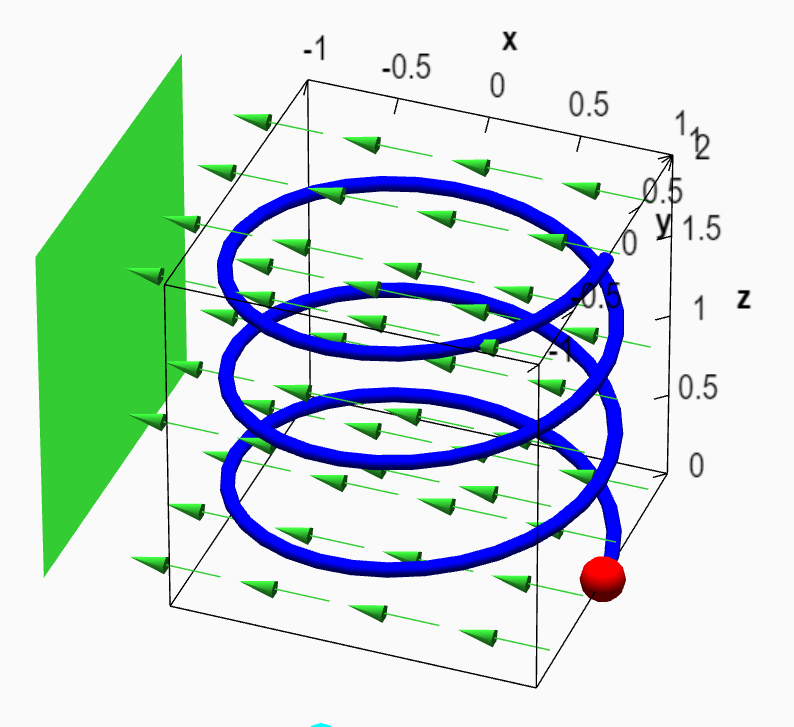
\includegraphics[width=0.8\textwidth, height = 200px]{Field_Helix.png}
	\\ $\textit{A very easy interpretation is to imagine the amount of work that a}$\\ $\textit{force field does on a particle as it moves along a curve.}$
	
	\item Imagine you have a Bead that is fixed to move along a helix defined as $c(t)$. The green rectangle is a magnet inducing a magnetic field $F(x,y,z)$(illustrated by the green arrows). The line integral of a vector field can be thought of, as work on the bead. 
	
	\item When the bead changes its position along the function, the force exorted by the magnetic field, and thus also the work, changes.\\
	
	Work is defined as $F\cdot s$ (force in direction of movement). For example, when the movement is 90 degrees from the direction of the force, the magnetic field does no work at all. So how can we get the direction of the bead? \\
	
	We just use its direction given by the velocity $c'(t)$. We denote the unit vector in the direction of the movement as $T(t) = \frac{c'(t)||}{c'(t)||}$. If you think of it, this absolutely makes sense as the derivate of $c(t)$ defines teh tangent vector to the path. 
	
	\item  The component of force in direction of the movement is simply the force of the magnetic field at a specific point on the function $c(t)$ along the tangent of $c(t)$: $F(c(t))\cdot T(t)$.(for future reference we will use$F\cdot T)$ \\
	
	Per definition we know that if we take the product of force and distance we get work. So $F\cdot T$ actually denotes the work per unit length along the helix. \\
	To get the total work we need to ake the line integral of this scalar-valued function. \\
	Work = $\int_{C}^{} F\cdot T ds$ (where C is the path along the function$c(t)$)
	
	\item To derive a final formula we go back to the first chapter where we looked at scalar-valued line integrals and take the end-formula that we derived.\\
	$\int_{C}^{} f ds = \int_{a}^{b} f(c(t))\cdot ||c'(t)|| dt$\\
	If we replace f with our new equation for work $F\cdot T$ we get:\\
	
	$\int_{C}^{} F\cdot T ds = \int_{a}^{b}F(c(t))\cdot T(t)\cdot ||c'(t)|| dt$\\
	
	We remember that we defined $T(t) =  \frac{c'(t)}{||c'(t)}$. If we replace $T(t)$ we get: \\
	
	$\int_{a}^{b}F\cdot T ds = \int_{a}^{b} F(c(t))\cdot\frac{c'(t)}{||c(t)||}\cdot ||c'(t)|| dt \\= \int_{a}^{b} = F(c(t))\cdot c'(t) dt = \int_{C}^{}F ds$.\\
	(because we usually write $T ds$ as ds.)
	\end{itemize}
	\newpage
	
	\section{Line integrals as circulation (Macroscopic)}
	\begin{itemize}
	
	\item In the previous chapter we learned how a vector field F over an oriented curve C "adds up" the component of the vector field that is tangential to the curve. In simple words, this defines how much the vector field is aligned with the curve. But what do we do if the curve is closed?
	
	\item The line inegral then indicates how much the vector fields tends to circulate around the curve C.\\
	$\int_{C}^{}F\cdot ds$ = $\oint_{C}^{}F\cdot ds$ (other notation) = circulation of F around C 
	\enlargethispage{\baselineskip}
	\item The circulation can be positive or negative according to the "circling"-direction of the vector field around the curve C. It is positive if it circles with the Curve and negative if it circles in counter-clockwise of the Curve.\\  $\newline$
	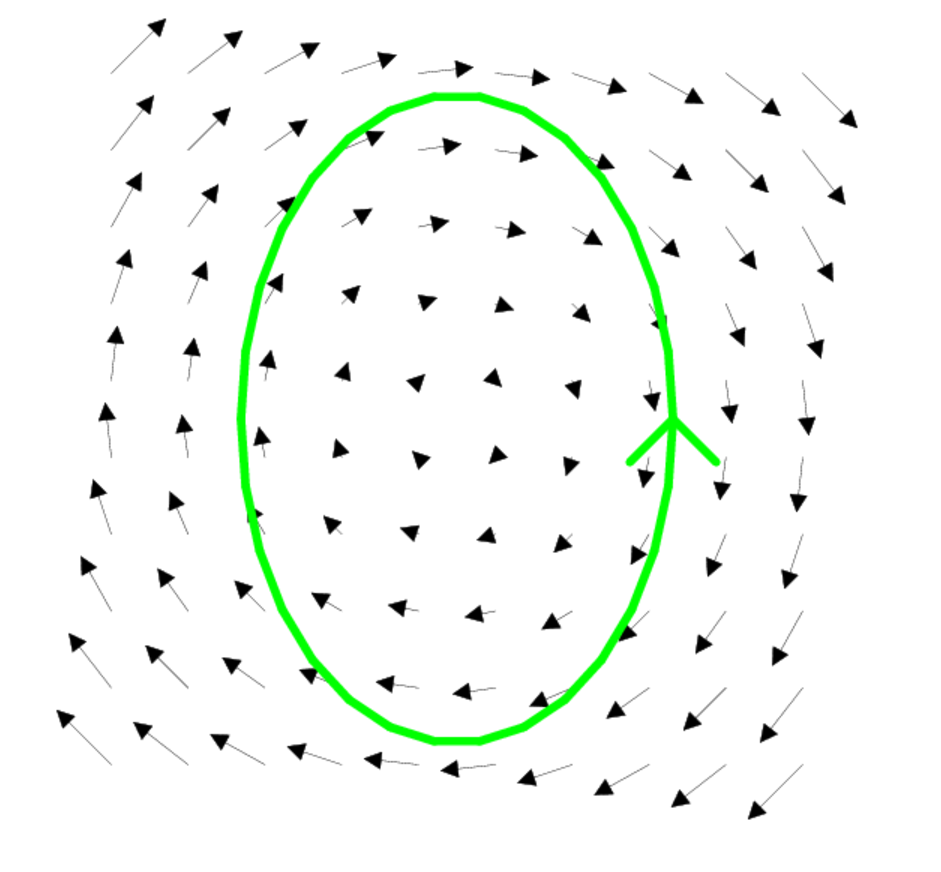
\includegraphics[width=0.8\textwidth, height = 200px]{circulation.png}
	
	$\textit{In this example the circulation of the vector field circulates clockwise in}$\\ $\textit{the opposite direction of the Curve.}$
	\newpage
	
	\section{The curl (Microscopic)}
	
	\newpage
	
	\section{Flux}
	
	\newpage
	
	\section{Divergence inkl. Divergenz Theorem}
	
	\newpage
	
	\section{Gradient Theorem}
	
	\newpage
	
	\section{Green's Theorem}
	
	\newpage
	
	\section{Stoke's Theorem}
	
	\newpage
	
	\section{Gauss Theorem}
	
	
	

	
	
	
	\end{itemize}
	

\end{document}